\documentclass[a4paper, 12pt]{article}
\usepackage[utf8]{inputenc}
\usepackage[T1, T2A]{fontenc}
\usepackage[a4paper, top=2cm, bottom=2cm, left=1cm, right=1cm, marginparwidth=1.75cm]{geometry}
\usepackage{graphicx}
\usepackage{amsmath}
\usepackage{amssymb}
\usepackage{amsfonts}
\usepackage{indentfirst}
\usepackage[english, russian]{babel}
\usepackage[section,above,below]{placeins}
\usepackage{pdfpages} 
\usepackage{svg}

\newcommand{\V}[1]{\int_Q #1(y) E(x-y) dy}
\newcommand{\R}[1]{\mathbb{R}^#1}
\newcommand{\ro}{ \tilde \rho_N}
\newcommand{\der}[2]{\dfrac{\partial #1}{\partial #2}}

\begin{document}
  
\subsubsection{Кратное интегрирование по областям с параметризуемой границей}
Пусть $Q$ -- область, по которой ведётся интегрирование, причём она имеет параметризуемую границу; $f$ -- функция под интегралом. Область можно разбить на сетку, например, следующим классическим способом (Рис. \ref{classic}, для простоты $Q$ --- круг).

{\bf Замечания}:
\begin{enumerate}
  \item На самом деле при интегрировании можно брать любой контур внутри кольца, но при специальном задании границ кольца в виде ${\bf r}(t,r)$ (на что рассчитывает метод) удобнее брать именно подобную кривую.
   \item Если нет возможности выразить функцию площади кольца $S_i=S(\tau_y,(i+0.5)\tau_y)$, в качестве площади при достаточно малых $\tau_y$ можно взять $S_i=\pi ((i+1)\tau_y)^2-\pi (i \tau_y)^2= \pi \tau^2_y (2i+1)$
   \item Как правило, при параметризации $t_0=0$, но $t_{\max}$ зависит от радиуса кривой $r=(i+0.5)\tau_y$, поэтому $\frac{1}{t_{\max}-t_0}$ не всегда является константным выражением и может быть вынесено за знак суммирования.
\item Для возможности равномерного интегрирования указанных криволинейных интегралов следует использовать естественную параметризацию.
\item Для круговой области вычислять кратный интеграл можно и классическими способами, однако если область имеет более сложную форму, классические методы будет чрезвычайно тяжело использовать. 
\end{enumerate}

{\bf Тесты.} На следующих рисунках (рисунки \ref{circ5}-\ref{hcirc2}) показаны результаты использования описанного метода интегрирования для разных областей и разных подинтегральных функций.
Области и функции взяты простыми, так как для сложных областей и функций трудно  аналитически найти интеграл, с которым требуется провести сравнение.
Замечено два типа поведения погрешности в зависимости от числа колец в интеграле: логарифмическое убывание и малое приближённо константное значение (на самом деле очень медленное логарифмическое убывание); при этом произведение {\it погрешность интегрирования} $\cdot$ {\it время вычислений} в первом случае логарифмически убывает, во втором --- логарифмически растёт.
Требуется также отметить, что графики рисовались в логарифмической шкале, поэтому точки с погрешностью не больше машинного нуля либо временем вычисления меньше машинного минимума --- не изображались. 

  
    \begin{figure}[h!]
      \noindent\centering{
      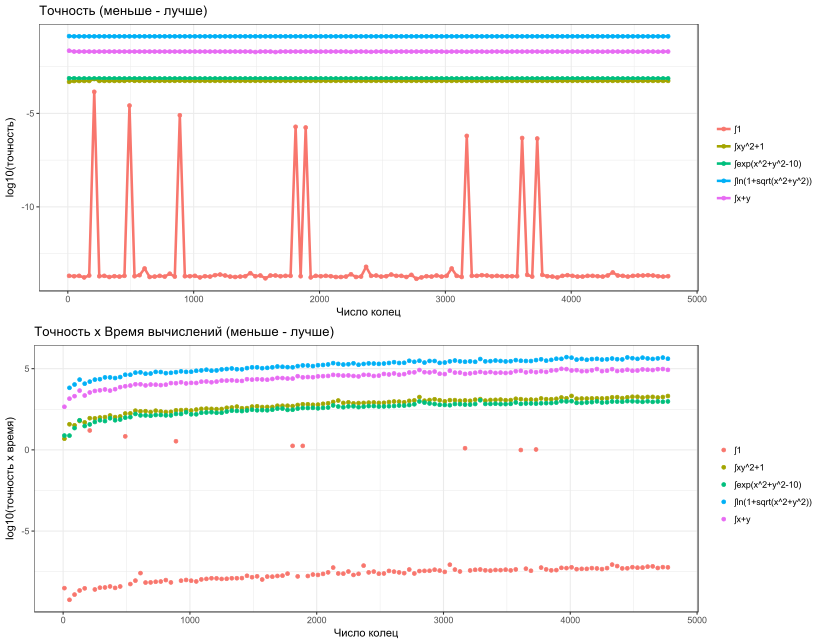
\includegraphics[width=\linewidth]{hcirc.pdf}
    }
      \caption{Точность и отношение точность-время от интегрирования для верхнего полукруга радиуса $r=2$}
      \label{hcirc2}
      \end{figure} 

      \begin{figure}[h] 
        \center{\begin{minipage}[h]{\linewidth} 
        \center{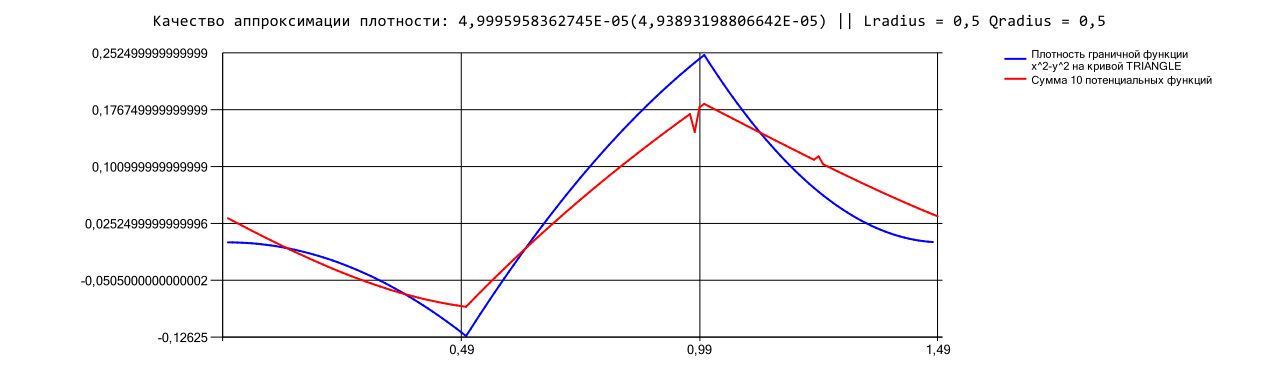
\includegraphics[width=0.6\linewidth]{d11.pdf} \\ для плотности} 
        \end{minipage}} 
        \vfill 
        \center{\begin{minipage}[h]{\linewidth} 
        \center{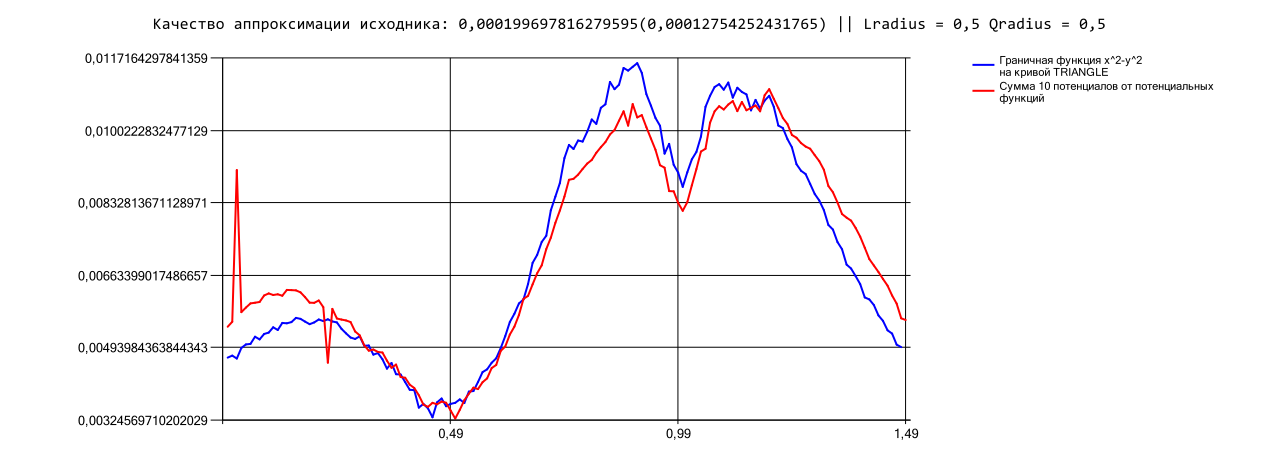
\includegraphics[width=0.6\linewidth]{v11.pdf} \\ для потенциала} 
        \end{minipage}} 
        \caption{Один из результатов работы алгоритма} 
        \label{hexampl2} 
        \end{figure}     
        
        \begin{figure}[h] 
          \center{\begin{minipage}[h]{\linewidth} 
          \center{\includegraphics[width=0.6\linewidth]{d12.pdf} \\ для плотности} 
          \end{minipage}} 
          \vfill 
          \center{\begin{minipage}[h]{\linewidth} 
          \center{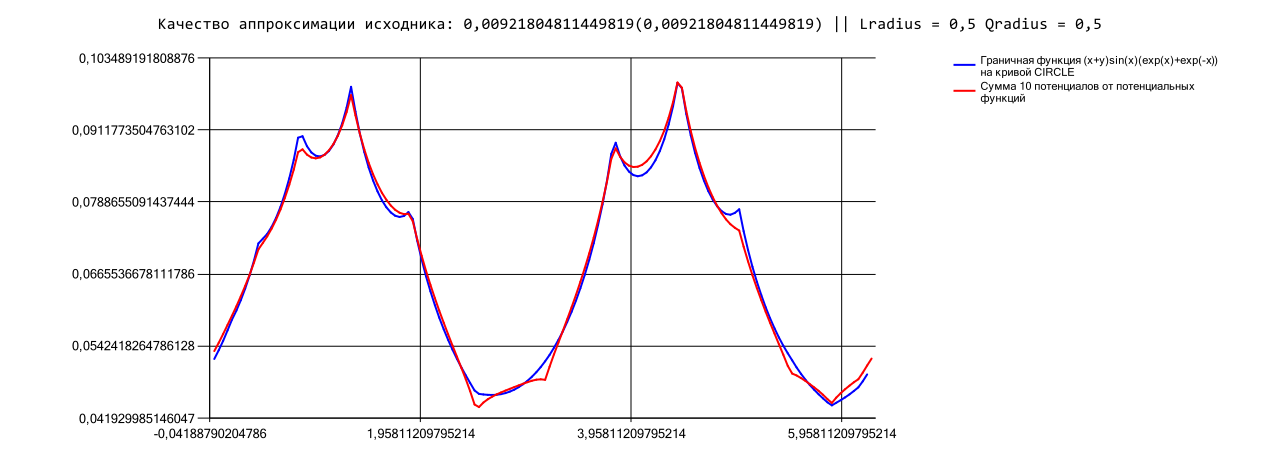
\includegraphics[width=0.6\linewidth]{v12.pdf} \\ для потенциала} 
          \end{minipage}} 
          \caption{Один из результатов работы алгоритма} 
          \label{ris:image1} 
          \end{figure}

          \begin{figure}[h] 
            \center{\begin{minipage}[h]{\linewidth} 
            \center{\includegraphics[width=0.6\linewidth]{d13.pdf} \\ для плотности} 
            \end{minipage}} 
            \vfill 
            \center{\begin{minipage}[h]{\linewidth} 
            \center{\includegraphics[width=0.6\linewidth]{v13.pdf} \\ для потенциала} 
            \end{minipage}} 
            \caption{Один из результатов работы алгоритма} 
            \label{p3} 
            \end{figure}

            \begin{figure}[h] 
              \center{\begin{minipage}[h]{\linewidth} 
              \center{\includegraphics[width=0.6\linewidth]{d14.pdf} \\ для плотности} 
              \end{minipage}} 
              \vfill 
              \center{\begin{minipage}[h]{\linewidth} 
              \center{\includegraphics[width=0.6\linewidth]{v14.pdf} \\ для потенциала} 
              \end{minipage}} 
              \caption{Один из результатов работы алгоритма} 
              \label{p4} 
              \end{figure}


\end{document}